\documentclass[english,notitlepage,reprint,nofootinbib]{revtex4-1}  % defines the basic parameters of the document

% if you want a single-column, remove reprint

% allows special characters (including æøå)
\usepackage[utf8]{inputenc}
\usepackage[english]{babel}

%% note that you may need to download some of these packages manually, it depends on your setup.
%% I recommend downloading TeXMaker, because it includes a large library of the most common packages.

\usepackage{physics,amssymb}  % mathematical symbols (physics imports amsmath)
\usepackage{graphicx}         % include graphics such as plots
\usepackage{xcolor}           % set colors
\usepackage{hyperref}         % automagic cross-referencing (this is GODLIKE)
\usepackage{tikz}             % draw figures manually
\usepackage{listings}         % display code
\usepackage{subfigure}        % imports a lot of cool and useful figure commands
\usepackage{lipsum}
\usepackage[ddmmyyyy]{datetime}
\usepackage{lmodern}

% (2) specify encoding
\usepackage[T1]{fontenc}
\usepackage{textcomp}
%\usepackage{unicode-math}
\usepackage{float}
\usepackage{balance}

% defines the color of hyperref objects
% Blending two colors:  blue!80!black  =  80% blue and 20% black
\hypersetup{ % this is just my personal choice, feel free to change things
    colorlinks,
    linkcolor={red!50!black},
    citecolor={blue!50!black},
    urlcolor={blue!80!black}}

%% Defines the style of the programming listing
%% This is actually my personal template, go ahead and change stuff if you want
\lstnewenvironment{python}{
	\lstset{ %
		inputpath=,
		backgroundcolor=\color{white!88!black},
		basicstyle={\ttfamily\tiny},
		commentstyle=\color{magenta},
		language=Python,
		morekeywords={True,False},
		tabsize=4,
		stringstyle=\color{green!55!black},
		frame=single,
		keywordstyle=\color{blue},
		showstringspaces=false,
		columns=fullflexible,
		keepspaces=true}
}{}

\lstnewenvironment{cpp}{
	\lstset{ %
		inputpath=,
		backgroundcolor=\color{white!88!black},
		basicstyle={\ttfamily\tiny},
		commentstyle=\color{magenta},
		language=C++,
		morekeywords={True,False},
		tabsize=4,
		stringstyle=\color{green!55!black},
		frame=single,
		keywordstyle=\color{blue},
		showstringspaces=false,
		columns=fullflexible,
		keepspaces=true}
}{}

\lstset{literate=
  {á}{{\'a}}1 {é}{{\'e}}1 {í}{{\'i}}1 {ó}{{\'o}}1 {ú}{{\'u}}1
  {Á}{{\'A}}1 {É}{{\'E}}1 {Í}{{\'I}}1 {Ó}{{\'O}}1 {Ú}{{\'U}}1
  {à}{{\`a}}1 {è}{{\`e}}1 {ì}{{\`i}}1 {ò}{{\`o}}1 {ù}{{\`u}}1
  {À}{{\`A}}1 {È}{{\'E}}1 {Ì}{{\`I}}1 {Ò}{{\`O}}1 {Ù}{{\`U}}1
  {ä}{{\"a}}1 {ë}{{\"e}}1 {ï}{{\"i}}1 {ö}{{\"o}}1 {ü}{{\"u}}1
  {Ä}{{\"A}}1 {Ë}{{\"E}}1 {Ï}{{\"I}}1 {Ö}{{\"O}}1 {Ü}{{\"U}}1
  {â}{{\^a}}1 {ê}{{\^e}}1 {î}{{\^i}}1 {ô}{{\^o}}1 {û}{{\^u}}1
  {Â}{{\^A}}1 {Ê}{{\^E}}1 {Î}{{\^I}}1 {Ô}{{\^O}}1 {Û}{{\^U}}1
  {œ}{{\oe}}1 {Œ}{{\OE}}1 {æ}{{\ae}}1 {Æ}{{\AE}}1 {ß}{{\ss}}1
  {ű}{{\H{u}}}1 {Ű}{{\H{U}}}1 {ő}{{\H{o}}}1 {Ő}{{\H{O}}}1
  {ç}{{\c c}}1 {Ç}{{\c C}}1 {ø}{{\o}}1 {å}{{\r a}}1 {Å}{{\r A}}1
  {€}{{\euro}}1 {£}{{\pounds}}1 {«}{{\guillemotleft}}1
  {»}{{\guillemotright}}1 {ñ}{{\~n}}1 {Ñ}{{\~N}}1 {¿}{{?`}}1
}

%% USEFUL LINKS:
%%
%%   UiO LaTeX guides:        https://www.mn.uio.no/ifi/tjenester/it/hjelp/latex/
%%   mathematics:             https://en.wikibooks.org/wiki/LaTeX/Mathematics

%%   PHYSICS !                https://mirror.hmc.edu/ctan/macros/latex/contrib/physics/physics.pdf

%%   the basics of Tikz:       https://en.wikibooks.org/wiki/LaTeX/PGF/TikZ
%%   all the colors!:          https://en.wikibooks.org/wiki/LaTeX/Colors
%%   how to draw tables:       https://en.wikibooks.org/wiki/LaTeX/Tables
%%   code listing styles:      https://en.wikibooks.org/wiki/LaTeX/Source_Code_Listings
%%   \includegraphics          https://en.wikibooks.org/wiki/LaTeX/Importing_Graphics
%%   learn more about figures  https://en.wikibooks.org/wiki/LaTeX/Floats,_Figures_and_Captions
%%   automagic bibliography:   https://en.wikibooks.org/wiki/LaTeX/Bibliography_Management  (this one is kinda difficult the first time)
%%   REVTeX Guide:             http://www.physics.csbsju.edu/370/papers/Journal_Style_Manuals/auguide4-1.pdf
%%
%%   (this document is of class "revtex4-1", the REVTeX Guide explains how the class works)


%% CREATING THE .pdf FILE USING LINUX IN THE TERMINAL
%%
%% [terminal]$ pdflatex template.tex
%%
%% Run the command twice, always.
%% If you want to use \footnote, you need to run these commands (IN THIS SPECIFIC ORDER)
%%
%% [terminal]$ pdflatex template.tex
%% [terminal]$ bibtex template
%% [terminal]$ pdflatex template.tex
%% [terminal]$ pdflatex template.tex
%%
%% Don't ask me why, I don't know.

\usepackage{thmtools}
\DeclareMathOperator{\nullspace}{Nul}
\DeclareMathOperator{\collspace}{Col}
\DeclareMathOperator{\rref}{Rref}
%%\DeclareMathOperator{\dim}{Dim}

 % "meq": must be equal
\newcommand{\meq}{\overset{!}{=}}

\newcommand{\R}{\mathbb{R}}
\newcommand*\Heq{\ensuremath{\overset{\kern2pt L'H}{=}}}
\usepackage{bm}
\newcommand{\uveci}{{\bm{\hat{\textnormal{\bfseries\i}}}}}
\newcommand{\uvecj}{{\bm{\hat{\textnormal{\bfseries\j}}}}}
\DeclareRobustCommand{\uvec}[1]{{%
  \ifcsname uvec#1\endcsname
     \csname uvec#1\endcsname
   \else
    \bm{\hat{\mathbf{#1}}}%
   \fi
}}
\usepackage[binary-units=true]{siunitx}

\makeatletter
\newcommand*{\balancecolsandclearpage}{%
  \close@column@grid
  \cleardoublepage
  \twocolumngrid
}
\makeatother

\newcounter{subproject}
\renewcommand{\thesubproject}{\alph{subproject}}
\newenvironment{subproj}{
\begin{description}
	\item[\refstepcounter{subproject}(\thesubproject)]
}{\end{description}}


\begin{document}
\title{Project 1 FYS3150}   % self-explanatory
\author{Anders P. Åsbø, Eivind Støland}               % self-explanatory

%\date{\today}
\noaffiliation                            % ignore this

\maketitle
\tableofcontents

\section{Introduction} \label{sec:I}

One of the most versatile tools in modern science is numerical integration, thus it it simportant to understand its limits. In this paper we have performed numerical integration of a second order differential equation. This was done by discretizing the differential equation, and formulating it as a matrix-vector equation. The matrix-vector equation was then solved using both a general, and specialized Thomas algorithm, as well as LU-decomposition. Under the pretext of solving a \(1\)D version of Poisson's equation, we have created and tested a numerical solver using the Thomas algorithm. Furthermore, we have compared our results with LU decomposition using the Armadillo library's solver. We measured the time spent by the various algorithms and their maximum relative error (to the analytic solution) in order to compare them quantitavely to see if they behave as expected.





\section{Formalism} \label{sec:II}

Poisson's equation is a well known equation from electromagnetism:

\begin{align*}
\nabla^2 \boldsymbol\Phi (\boldsymbol r) &= -4\pi \rho (\boldsymbol r) \, ,
\end{align*}

where $\boldsymbol r$ is the position, $\rho(\boldsymbol r)$ is the charge density, and $\boldsymbol \Phi (\boldsymbol r)$ is the electrostatic potential. If we assume spherical symmetry, this simplifies into a one-dimensional equation:

\begin{align*}
\frac{1}{r^2} \frac{d}{dr} \bigg(r^2 \frac{d\boldsymbol \Phi}{dr} \bigg) = - 4\pi \rho \, ,
\end{align*}

where $r = |\boldsymbol r|$. We can substitute $\boldsymbol \Phi (r) = \phi(r)/r$, which gives us:

\begin{align*}
\frac{d^2 \phi}{dr^2} = - 4\pi r \rho (r)
\end{align*}

This is a second order differential equation which can be written generally as:

\begin{align*}
-u''(x) = f(x) \, ,
\end{align*}

where we have changed $r \to x$, $\phi \to u$ and $4\pi r \rho \to f(x)$. In order to proceed we need to pick a specific sample problem to be used. We choose to solve this equation with Dirichlet boundary conditions, meaning that $x \in (0,1)$ and $u(0)=u(1)=0$. As for the source term $f$ we choose $f(x) = 100 e^{-10 x}$. This has the advantage of being possible to solve analytically:

\begin{align*}
-u''(x) &= f(x) \\
-u''(x) &= 100 e^{-10x} \\
-u'(x) &= -10e^{-10x} - C \\
-u(x) &= e^{-10x} - Cx - D \\
u(x) &= Cx + D - e^{-10x} \, ,
\end{align*}

where $C$ and $D$ are arbitrary constants. We use the boundary conditions in order to determine them:

\begin{align*}
u(0) &= 0 \\
\implies D - 1 &= 0 \\
D &= 1 \\
u(1) &= 0 \\
\implies C + 1 - e^{-10} &= 0 \\
C &= -(1 - e^{-10})
\end{align*}

All in all this gives us that:

\begin{align*}
u(x) &= 1 - (1 - e^{-10}) x - e^{-10x}
\end{align*}

Now we have an analytical solution we can compare our numerical solutions to later.

In order to solve the problem numerically we first need some definitions in order. We discretize with the grid points given by $x_i = ih$, in the interval from $x_0 = 0$ to $x_{n+1} = 1$. The step length is then given by $h = 1/(n+1)$. We name the discretized approximation to the solution $v_i$. We can then approximate the second derivative of $u$ as:

\begin{align*}
- \frac{v_{i+1} + v_{i-1} - 2v_i}{h^2} &= f_i \, ,
\end{align*}

where $f_i = f(x_i)$ and $i = 1,...,n$. We look at some terms separately in order to find the matrix-vector form of this problem. First we look at the expression at the boundaries, starting with $i=1$:

\begin{align*}
-\frac{v_2 + v_0 - 2v_1}{h^2} &= f_1 \\
2v_1 - v_2 &= h^2 f_1 \\
2v_1 - v_2 &= \tilde{b}_1 \, ,
\end{align*}

where we have defined a new variable $\tilde{b}_i = h^2 f_i$ and applied the relevant boundary condition. We then look at the expression when $i=n$:

\begin{align*}
-\frac{v_{n+1} + v_{n-1} - 2v_{n}}{h^2} &= f_n \\
-v_{n-1} + 2v_n &= \tilde{b}_n \, ,
\end{align*}

where we also applied the relevant boundary condition. The general expression can also be rewritten as:

\begin{align*}
-v_{i-1} + 2v_i - v_{i+1} &= \tilde{b}_i
\end{align*}

This now clearly takes the shape of a matrix-vector problem. We define a vector $\textbf{v}$ which contains all the $v_i$ and similarly a vector $\tilde{\textbf{b}}$ which contains all the $b_i$. The coefficients on the left-hand side of the equations determine a $n\times n$-matrix \textbf{A}:

\begin{align*}
\textbf{A} &= \begin{bmatrix}
2 & -1 & 0 & ... & ... & 0 \\
-1 & 2 & -1 & 0 & ... & ... \\
0 & -1 & 2 & -1 & 0 & ... \\
... & ... & ... & ... & ... & ... \\
0 & ... & ... & -1 & 2 & -1 \\
0 & ... & ... & 0 & -1 & 2
\end{bmatrix}
\end{align*}

The matrix-vector problem we need to solve then is:

\begin{align*}
\textbf{A}\textbf{v} &= \tilde{\textbf{b}}
\end{align*}

\textbf{A} is a tridiagonal matrix. This means we can apply methods specialized for this kind of linear algebra problem. A tridiagonal matrix can be decomposed into three vectors, one for the diagonal and one each for the bands above and below the diagonal. We choose the vectors \textbf{a}, \textbf{b} and \textbf{c}. Their components are defined the following way:

\begin{align*}
\textbf{A} &= \begin{bmatrix}
b_1 & c_1 & 0 & ... & ... & 0 \\
a_2 & b_2 & c_2 & 0 & ... & ... \\
0 & a_3 & b_3 & c_3 & 0 & ... \\
... & ... & ... & ... & ... & ... \\
0 & ... & ... & a_{n-1} & b_{n-1} & c_{n-1} \\
0 & ... & ... & 0 & a_{n} & b_n
\end{bmatrix}
\end{align*}

As the bands above and below the diagonal have one element less than the diagonal itself, we note that \textbf{a} and \textbf{c} both have $n-1$ elements defined this way instead of $n$ elements (as \textbf{b}). We choose, however, to let \textbf{a}'s first component to be denoted $a_2$, as the indexing then matches those along the same row of the matrix \textbf{A}.

In general this gives us equations on the form:

\begin{align*}
a_i v_{i-1} + b_i v_i + c_i v_{i+1} &= \tilde{b}_i \, ,
\end{align*}

which we need to solve. As there is not element $c_n$ or $a_1$, we simply define them to be 0 instead, and thus the equation is valid from $i = 1,...,n$. Looking at the tridiagonal matrix \textbf{A} with general elements again, we can see that we can eliminate the band below the diagonal (the components of \textbf{a}). First we take the first row multiplied by $a_2/b_1$ and subtract it from row 2. This leaves us with the following matrix:

\begin{align*}
\textbf{A} &= \begin{bmatrix}
b_1 & c_1 & 0 & ... & ... & 0 \\
0 & b_2 - \frac{a_2c_1}{b_1} & c_2 & 0 & ... & ... \\
0 & a_3 & b_3 & c_3 & 0 & ... \\
... & ... & ... & ... & ... & ... \\
0 & ... & ... & a_{n-1} & b_{n-1} & c_{n-1} \\
0 & ... & ... & 0 & a_{n} & b_n
\end{bmatrix}
\end{align*}

We now define $\tilde{d}_2 = b_2 - \frac{a_2c_1}{b_1}$, and $\tilde{d}_1$ in order to simplify further equations:

\begin{align*}
\textbf{A} &= \begin{bmatrix}
\tilde{d}_1 & c_1 & 0 & ... & ... & 0 \\
0 & \tilde{d}_2 & c_2 & 0 & ... & ... \\
0 & a_3 & b_3 & c_3 & 0 & ... \\
... & ... & ... & ... & ... & ... \\
0 & ... & ... & a_{n-1} & b_{n-1} & c_{n-1} \\
0 & ... & ... & 0 & a_{n} & b_n
\end{bmatrix}
\end{align*}

We can now similarly eliminate $a_3$ by multiplying row 2 with $\frac{a_3}{\tilde{d}_2}$ and subtract this from row 3. This gives us the following:

\begin{align*}
\textbf{A} &= \begin{bmatrix}
\tilde{d}_1 & c_1 & 0 & ... & ... & 0 \\
0 & \tilde{d}_2 & c_2 & 0 & ... & ... \\
0 & 0 & b_3 - \frac{a_3 c_2}{\tilde{d}_2} & c_3 & 0 & ... \\
... & ... & ... & ... & ... & ... \\
0 & ... & ... & a_{n-1} & b_{n-1} & c_{n-1} \\
0 & ... & ... & 0 & a_{n} & b_n
\end{bmatrix}
\end{align*}

We now define $\tilde{d}_3 = b_3 - \frac{a_3c_2}{\tilde{d}_2}$. This process can be repeated until all the elements in the band below the diagonal are eliminated. The new diagonal elements ($\tilde{d}_i$) are given by the following formula:

\begin{align*}
\tilde{d}_i &= b_i - \frac{a_i c_{i-1}}{\tilde{d}_{i-1}} \quad , \quad i = 2,...,n \, ,
\end{align*}

with $\tilde{d}_1 = b_1$. This leaves us with a new matrix \textbf{A}:

\begin{align*}
\textbf{A} &= \begin{bmatrix}
\tilde{d}_1 & c_1 & 0 & ... & ... & 0 \\
0 & \tilde{d}_2 & c_2 & 0 & ... & ... \\
0 & 0 & \tilde{d}_3 & c_3 & 0 & ... \\
... & ... & ... & ... & ... & ... \\
0 & ... & ... & 0 & \tilde{d}_{n-1} & c_{n-1} \\
0 & ... & ... & 0 & 0 & \tilde{d}_n
\end{bmatrix}
\end{align*}


Now in order for us to use this to solve the problem, it also needs to be applied to $\tilde{\textbf{b}}$ simultaneously, resulting in a new vector $\tilde{\textbf{f}}$ with elements given as:

\begin{align*}
\tilde{f}_i &= \tilde{b}_i - \frac{a_i \tilde{f}_{i-1}}{\tilde{d}_{i-1}} \quad , \quad i = 2,...,n \, ,
\end{align*}

with $\tilde{f}_1 = \tilde{b}_1$. This gives us equations on the following form that we need to solve:

\begin{align*}
\tilde{d}_i v_i  + c_i v_{i+1} = \tilde{f}_i \quad , \quad i = 1,...,n
\end{align*}

We note that $c_n = 0$, which means that when $i=n$, we have that:

\begin{align*}
\tilde{d}_n v_n &= \tilde{f}_n \\
v_n &= \frac{\tilde{f}_n}{\tilde{d}_n}
\end{align*}

Now that we know one value \textbf{v}, this will now uniquely determine the other elements. We can see this by rewriting:

\begin{align*}
\tilde{d}_i v_i  + c_i v_{i+1} &= \tilde{f}_i \\
v_i &= \frac{\tilde{f}_i - c_i v_{i+1}}{\tilde{d}_i}
\end{align*}

As long as we know the last element in \textbf{v} (which we do at this point) this relation allows us to find $v_i$ for $i = n-1,...,1$. As we run through the elements from the largest $i$ to the smallest we call this part the backwards substitution part. For similar reasons we call calculating the $\tilde{d}_i$ and $\tilde{f}_i$ the forwards substitution part. This algorithm is called the Thomas algorithm \citep{Thomas1949} and is used for solving a general tridiagonal matrix. In our case however, we know what the elements of \textbf{A} are, allowing us to form a special algorithm. First we look at the $\tilde{d}_i$:

\begin{align*}
\tilde{d}_i &= b_i - \frac{a_i c_{i-1}}{\tilde{d}_{i-1}}
\end{align*}

We recognize that $b_i = 2$, and $a_i = c_{i-1} = i-1$. This simplifies the equation:

\begin{align*}
\tilde{d}_i &= 2 - \frac{1}{\tilde{d}_{i-1}} \\
&= \frac{i+1}{i}
\end{align*}

We can simplify $\tilde{f}_i$ in a similar way:

\begin{align*}
\tilde{f}_i &= \tilde{b}_i - \frac{a_i \tilde{f}_{i-1}}{\tilde{d}_{i-1}} \\
\tilde{f}_i &= \tilde{b}_i + \frac{i-1}{i}\tilde{f}_{i-1}
\end{align*}

This also gives us a simplification for $v_i$:

\begin{align*}
v_i &= \frac{\tilde{f}_i - c_i v_{i+1}}{\tilde{d}_i} \\
&= \frac{i}{i+1}(\tilde{f}_i + v_{i+1})
\end{align*}

This can be optimized somewhat, which will be discussed in section III. Further details on the topics discussed in this section and on LU decomposition can be found in \citep{Hjorth-Jensen2015}.

\newpage


\section{Implementation} \label{sec:III}
The general Thomas algorithm is implemented directly in two C++ functions. The first is a function performing the forward substitution:
\begin{cpp}
void general_forward(vec& a, vec& b, vec& c, vec& b_twiddle, int N)
{
  double decomp_factor = 0;
  //forward loop
  for (int i = 1; i<N; ++i){
    decomp_factor = a[i-1]/b[i-1];  // precalculate to get 5N FLOPS
    b[i] = b[i] - c[i-1]*decomp_factor;
    b_twiddle[i] = b_twiddle[i] - b_twiddle[i-1]*decomp_factor;
  }
}
\end{cpp}
Followed by a function performing the backwards substitution:
\begin{cpp}
void general_backward(vec& b, vec& b_twiddle, vec& c, vec& u, int N)
{
  //setting first element
  u[N-1] = b_twiddle[N-1]/b[N-1];

  //backward loop
  for (int i = N-1; i>=1;--i){
    u[i-1] = (b_twiddle[i-1] - c[i-1]*u[i])/b[i-1];
  }
}
\end{cpp}
The vectors \verb+a+, \verb+b+ and \verb+c+ stores the lower, middle, and upper diagonals of the Toeplitz matrix respectivly. \verb+b_twiddle+ is the solution vector to the vector equation from which the algorithm is derived, \verb+u+ is the unknown vector we are solving for, and \verb+N+ is the dimention of the Toeplitz matrix. The forward substitiution, as first presented, requires \(6(N-1)\approx 6N\) floating point operations (FLOPs) to complete. In "\verb+general_forward+", the factor \(a_{i-1}/b_{i-1}\) is precalculated each iteration, thus reducing the number of FLOPS to \(5(N-1)\approx 5N\). The backward substitution requires \(3(N-1)+1 = 3N\) FLOPs to complete, thus the general algorithm requires \(8N\) FLOPs to complete fully.

During forward substitution, the vector \verb+b+ is overwritten with the resulting \(\tilde{d}_{i}\) values, since there is no dependence on previous diagonal elements. Vector \verb+b_twiddle+ is similarly overwritten with the resulting \(\tilde{f}_{i}\) values. This, combined with passing the vectors by reference, reduces the amount of allocated memory by \(2N\cdot \SI{64}{\bit}\)s for a total of \(5N\cdot \SI{64}{\bit}\)s of memory used by the general algorithm.

The specialized Thomas algorithm is similarly implemented in two functions. The forward substitution:
\begin{cpp}
void special_forward(vec& b_recip, vec& b_twiddle, int N)
{
  //forward loop
  for (int i = 1; i<N; ++i){
    b_twiddle[i] = b_twiddle[i] + b_twiddle[i-1]*b_recip[i-1];
  }
}
\end{cpp}
The backwards substitution:
\begin{cpp}
void special_backward(vec& b_recip, vec& b_twiddle, vec& u, int N)
{
  //setting first element
  u[N-1] = b_twiddle[N-1]/b_recip[N-1];

  //backward loop
  for (int i = N-1; i>=1; --i){
    u[i-1] = (b_twiddle[i-1] + u[i])*b_recip[i-1];
  }
}
\end{cpp}
For the specialized algorithm, the reciprocals of the new diagonal elements are precalculated as:

\begin{align*}
\frac{1}{\tilde{d}_{i}} = \frac{i}{i+1}\text{ for } i=1,2,3,...N,
\end{align*}

and passed to "\verb+special_forward+" and "\verb+special_backward+", by reference, as the vector \verb+b_recip+. This precalculation takes \(2N\) FLOPs. The forward substitution takes \(2(N-1)\approx 2N\) FLOPs. The backwards substitution takes \(2(N-1)+1 = 2N\) FLOPs. As such, the specialized implementation takes a total of \(6N\) FLOPs. During forward substitution, vector \verb+b_twiddle+ is overwritten with the resulting \(\tilde{f}_{i}\) values. The total memory allocated by the specialized algorithm is \(3N\cdot \SI{64}{\bit}\)s.

The LU decomposition was implemented using the Armadillo library's built in functions:
\begin{cpp}
  // LU decomposition with armadillo
  lu(L,U,A);

  // Solving resulting equation sets
  vec y = solve(L,b_twiddle);
  vec u = solve(U,y);
\end{cpp}
The matrices \verb+L+, \verb+U+, \verb+A+ store the lower triangular, upper triangular, and toeplitz matrix respectivly. The vector \verb+y+ contains the solution to
\begin{align*}
\textbf{Ly} = \tilde{\textbf{b}},
\end{align*}
and the vector \verb+u+ contains the unknown values once the LU decomposition is complete. The computational cost of LU decomposition is on the order of \(\frac{2}{3}N^{3}\)FLOPs \citep{Hjorth-Jensen2018}. The LU decomposition requires the allocation of three \(N\times N\) matrices, and thus the memory needed for the matrices alone is \(3N^{2} \cdot \SI{64}{\bit}\)s.

Our implementation runs all the solvers sequentally. Each solver only allocates the memory it needs to perform its algorithm, and writes the results to binary files, before deallocating memory. The entire C++ program \hyperref[A]{(see appendix A)} runs the three solvers for one value of \(N\). The Python-script "\verb+data_analysis.py+" builds (if necessary) and runs the C++ program for given values of \(N\). The Python-script reads in the data from the binary files, and takes care of plotting and error analysis. For a more detaild explanation, see the readme-file at the repository linked in \hyperref[A]{appendix A}. For the specifications of the benchmark system, see \hyperref[B]{appendix B}.

\newpage

\section{Analysis} \label{sec:IV}
\subsection{Plots of the general Thomas algorithm} \label{subsec:IV:A}

We ran the Thomas algorithm with $N=10$, $N=10^2$, and $N=10^3$ steps and created plots of the resulting data, and compared this with the analytic solution. These plots can be found in figures \hyperref[fig:iv:a:1]{1}, \hyperref[fig:iv:a:2]{2} and \hyperref[fig:iv:a:3]{3}.


\begin{figure}[H]
	\centering
	\label{fig:iv:a:1}
	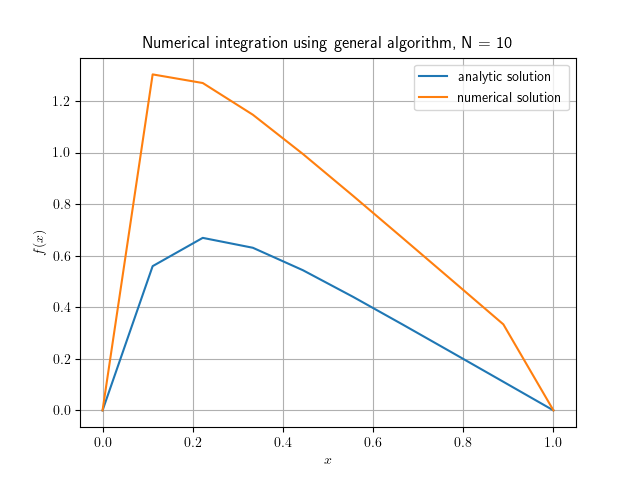
\includegraphics[width=\columnwidth]{plots/Figure_1.png}
	\caption{Plot of numerical and analytical solution, using the general Thomas algorithm with
	\(N=10^{1}\).}
\end{figure}

\begin{figure}[H]
	\centering
	\label{fig:iv:a:2}
	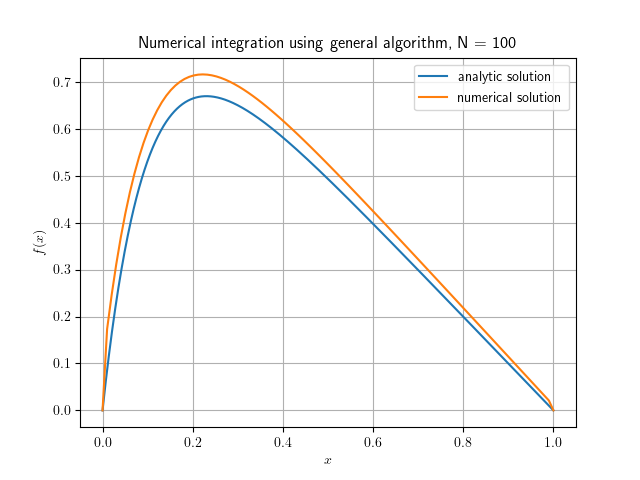
\includegraphics[width=\columnwidth]{plots/Figure_2.png}
	\caption{Plot of numerical and analytical solution, using the general Thomas algorithm with
	\(N=10^{2}\).}
\end{figure}

\begin{figure}[H]
	\centering
	\label{fig:iv:a:3}
	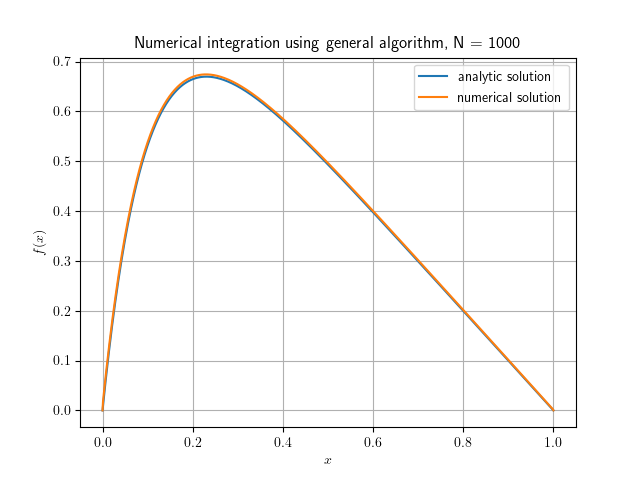
\includegraphics[width=\columnwidth]{plots/Figure_3.png}
	\caption{Plot of numerical and analytical solution, using the general Thomas algorithm with
	\(N=10^{3}\).}
\end{figure}


As expected we see that for larger $N$ (shorter step length) the numerical approximation is closer to the analytic one, which also suggests that the algorithm is working as intended.


\subsection{Relative errors} \label{subsec:IV:B}

We measured the logarithm with base 10 of the maximum relative error for each algorithm for several $N$, and recorded the results in \hyperref[table:iv:b:1]{table I}. The variable $\epsilon$ in this table was calculated using the following formula:

\begin{align*}
\epsilon &= \max\bigg\{\log_{10} \bigg( \bigg| \frac{v_i-u_i}{u_i} \bigg| \bigg)\bigg\} \, ,
\end{align*} 

and as such it indicates the maximum relative error in a single run of an algorithm.


\begin{table}[H]
	\label{table:iv:b:1}
	\caption{Table with \(\log_{10}\) of relative error for general and special Thomas algorithms, LU decomposition, and \(\log_{10}\) of step size \(h\). To run the LU decomposition with $N \geq 10^5$ would have required more memory than we have available, and have thus not been performed.}

	\begin{tabular}{|c|c|c|c|c|}
	\hline
		\(\log_{10}(h)\): & \(\epsilon\) General & \(\epsilon\) Special & \(\epsilon\) LU & \(N\) \\\hline
		\(\num{-1.04139e+00}\) & \(\num{3.02620e-01}\) & \(\num{3.60131e-01}\) & \(\num{3.0262e-01}\) & \(10^{1}\) \\
		\(\num{-2.00432e+00}\) & \(\num{3.42630e-02}\) & \(\num{4.24989e-02}\) & \(\num{3.4263e-02}\) & \(10^{2}\) \\
		\(\num{-3.00043e+00}\) & \(\num{3.47475e-03}\) & \(\num{4.33859e-03}\) & \(\num{3.4748e-03}\) & \(10^{3}\) \\
		\(\num{-4.00004e+00}\) & \(\num{3.47972e-04}\) & \(\num{4.34783e-04}\) & \(\num{3.4797e-04}\) & \(10^{4}\) \\
		\(\num{-5.00000e+00}\) & \(\num{3.48018e-05}\) & \(\num{4.34876e-05}\) & - & \(10^{5}\) \\
		\(\num{-6.00000e+00}\) & \(\num{4.21013e-06}\) & \(\num{4.34875e-06}\) & - & \(10^{6}\) \\
		\(\num{-7.00000e+00}\) & \(\num{1.00517e-06}\) & \(\num{4.34397e-07}\) & - & \(10^{7}\) \\
		\(\num{-8.00000e+00}\) & \(\num{-1.14050e-03}\) & \(\num{3.76530e-08}\) & - & \(10^{8}\) \\\hline
	\end{tabular}

\end{table}

\subsection{Benchmarks} \label{subsec:IV:C}

We measured execution time for the three algorithms (for various amounts of steps), in order to compare the time spent by each to see if everything behaves as expected. The results are shown in \hyperref[table:iv:c:1]{table II}. We expected that the the slowest of the three would be the LU decomposisition, as that is a method used to solve general matrix-vector equations. The general Thomas algorithm should be quicker, as that is dependent on the matrix being tridiagonal, and the special Thomas algorithm should be the fastest of the three, as it is reliant on the elements also having specific values. We can see from the execution times listed in \hyperref[table:iv:c:1]{table II} that these expectations were met. The LU decomposition is the slowest, the general Thomas algorithm is quicker, and the special Thomas algorithm is the quickest one, for all amounts of steps used. Note that for $N=10$ the execution time for the specialized and general algorithm is the same, which is also the same as the execution time for the specialized algorithm with $N=10^2$ steps. This probably has something to do with precision in the measurement of the execution time, and seems to suggest that $1 \times 10^{-6}\, s$ is the shortest time interval we can measure, as the special algorithm should be faster with $N=10$ steps than with $N=10^2$ steps (for obvious reasons).


\begin{table}[H]
	\centering
	\label{table:iv:c:1}
	\caption{Table of execution time in seconds for general and special Thomas algorithms, and LU decomposition.}

	\begin{tabular}{|c|c|c|}
		\hline
		Algorithm & Execution time \([s]\) & \(N\) \\\hline
		General Thomas & \(\num{1e-06}\) & \(10^{1}\) \\
		General Thomas & \(\num{3e-06}\) & \(10^{2}\) \\
		General Thomas & \(\num{1.8e-05}\) & \(10^{3}\) \\
		General Thomas & \(\num{0.000119}\) & \(10^{4}\) \\\hline
		Specialized Thomas & \(\num{1e-06}\) & \(10^{1}\) \\
		Specialized Thomas & \(\num{1e-06}\) & \(10^{2}\) \\
		Specialized Thomas & \(\num{7e-06}\) & \(10^{3}\) \\
		Specialized Thomas & \(\num{4.6e-05}\) & \(10^{4}\) \\\hline
		LU decomposition & \(\num{0.000309}\) & \(10^{1}\) \\
		LU decomposition & \(\num{0.000755}\) & \(10^{2}\) \\
		LU decomposition & \(\num{0.171256}\) & \(10^{3}\) \\
		LU decomposition & \(\num{158.701}\) & \(10^{4}\) \\\hline
	\end{tabular}

\end{table}

\section{Conclusion} \label{sec:V}

\bibliography{kilder}{}

\appendix
\section{Source code} \label{A}
All code for this report was written in C++ and Python 3.8, and the complete set of files can be found at \url{https://github.com/FunkMarvel/FYS3150_Project_1.git}

\section{System specifications} \label{B}
The all results included in this report were achieved by running the implementation on the following system:
\begin{itemize}
	\item CPU: AMD Ryzen \(9\) \(3900\)X
	\item RAM: \(2\times\SI{8}{\giga\byte}\) Corsair Vengeance LPX DDR\(4\) \(\SI{3200}{\mega\hertz}\)
\end{itemize}

\end{document}
